%%
%% Beginning of file 'sample.tex'
%%
%% Modified 2015 December
%%
%% This is a sample manuscript marked up using the
%% AASTeX v6.x LaTeX 2e macros.

%% AASTeX is now based on Alexey Vikhlinin's emulateapj.cls 
%% (Copyright 2000-2015).  See the classfile for details.
%%
%% AASTeX requires revtex4-1.cls (http://publish.aps.org/revtex4/) and
%% other external packages (latexsym, graphicx, amssymb, longtable, and epsf).
%% All of these external packages should already be present in the modern TeX 
%% distributions.  If not they can also be obtained at www.ctan.org.

%% The first piece of markup in an AASTeX v6.x document is the \documentclass
%% command. LaTeX will ignore any data that comes before this command. The 
%% documentclass can take an optional argument to modify the output style.
%% The command below calls the preprint style  which will produce a tightly 
%% typeset, one-column, single-spaced document.  It is the default and thus
%% does not need to be explicitly stated.
%%

%% using aastex version 6
\documentclass[onecolumn]{aastex6}
\usepackage{subfigure}
\usepackage{amsmath}
\usepackage{listings}
\usepackage{color}
 
\definecolor{codegreen}{rgb}{0,0.6,0}
\definecolor{codegray}{rgb}{0.5,0.5,0.5}
\definecolor{codepurple}{rgb}{0.58,0,0.82}
\definecolor{backcolour}{rgb}{0.95,0.95,0.92}
 
\lstdefinestyle{mystyle}{
    backgroundcolor=\color{backcolour},   
    commentstyle=\color{codegreen},
    keywordstyle=\color{magenta},
    numberstyle=\tiny\color{codegray},
    stringstyle=\color{codepurple},
    basicstyle=\footnotesize,
    breakatwhitespace=false,         
    breaklines=true,                 
    captionpos=b,                    
    keepspaces=true,                 
    numbers=left,                    
    numbersep=5pt,                  
    showspaces=false,                
    showstringspaces=false,
    showtabs=false,                  
    tabsize=2
}
 
\lstset{style=mystyle}


%% The other main article choice is a tightly typeset, two-column article
%% that more closely resembles the final typeset pdf article.
%%
%% \documentclass[twocolumn]{aastex6}
%% 
%% There are other optional arguments one can envoke to allow other 
%% actions. 
%%
% These are the available options:
%   manuscript	: onecolumn, doublespace, 12pt fonts
%   preprint	: onecolumn, single space, 10pt fonts
%   preprint2	: twocolumn, single space, 10pt fonts
%   twocolumn	: a two column article. Probably not needed, but here just in case.
%   onecolumn	: a one column article; default option.
%   twocolappendix: make 2 column appendix
%   onecolappendix: make 1 column appendix is the default. 
%   astrosymb	: Loads Astrosymb font and define \astrocommands. 
%   tighten	: Makes baselineskip slightly smaller
%   times	: uses times font instead of the default
%   linenumbers	: turn on lineno package.
%   trackchanges : required to see the revision mark up and print output
%   numberedappendix: Labels appendix sections A, B, ... This is the default.
%   appendixfloats: Needed. Resets figure and table counters to zero

%% these can be used in any combination, e.g.
%%
%% \documentclass[twocolumn,twocolappendix,linenumbers,trackchanges]{aastex6}

%% If you want to create your own macros, you can do so
%% using \newcommand. Your macros should appear before
%% the \begin{document} command.
%%
\newcommand{\vdag}{(v)^\dagger}
\newcommand\aastex{AAS\TeX}
\newcommand\latex{La\TeX}

%% AASTeX 6.0 supports the ability to suppress the names and affiliations
%% of some authors and displaying them under a "collaboration" banner to
%% minimize the amount of author information that to be printed.  This 
%% should be reserved for articles with an extreme number of authors.
%%
%% Mark up commands to limit the number of authors on the front page.
\AuthorCallLimit=2
%% Will only show Schwarz & Muench since Schwarz and Muench
%% are in the same \author call. 
\fullcollaborationName{The Friends of AASTeX Collaboration}
%% will print the collaboration text after the shortened author list.
%% These commands have to COME BEFORE the \author calls.
%%
%% Note that all of these author will be shown in the published article.
%% This feature is meant to be used prior to acceptance to make the
%% front end of a long author article more manageable.
%% Use \allauthors at the manuscript end to show the full author list.

%% The following command can be used to set the latex table counters.  It
%% is needed in this document because it uses a mix of latex tabular and
%% AASTeX deluxetables.  In general it should not be needed.
%\setcounter{table}{1}

%%%%%%%%%%%%%%%%%%%%%%%%%%%%%%%%%%%%%%%%%%%%%%%%%%%%%%%%%%%%%%%%%%%%%%%%%%%%%%%%
%%
%% The following commented section outlines numerous optional output that
%% can be displayed in the front matter or as running meta-data.
%%
%% You can insert a short comment on the title page using the command below.
%% \slugcomment{Not to appear in Nonlearned J., 45.}
%%
%% If you wish, you may supply running head information, although
%% this information may be modified by the editorial offices.
%%\shorttitle{\aastex sample article}
%%\shortauthors{Schwarz et al.}
%%
%% You can add a light gray and diagonal water-mark to the first page 
%% with this command:
%% \watermark{text}
%% where "text", e.g. DRAFT, is the text to appear.  If the text is 
%% long you can control the water-mark size with:
%% \setwatermarkfontsize{dimension}
%% where dimension is any recognized LaTeX dimension, e.g. pt, in, etc.
%%
%%%%%%%%%%%%%%%%%%%%%%%%%%%%%%%%%%%%%%%%%%%%%%%%%%%%%%%%%%%%%%%%%%%%%%%%%%%%%%%%

%% This is the end of the preamble.  Indicate the beginning of the
%% paper itself with \begin{document}.

\begin{document}

%% LaTeX will automatically break titles if they run longer than
%% one line. However, you may use \\ to force a line break if
%% you desire.

\title{HW 03: An Eclipsing Binary in the LMC}

%% Use \author, \affil, plus the \and command to format author and affiliation 
%% information.  If done correctly the peer review system will be able to
%% automatically put the author and affiliation information from the manuscript
%% and save the corresponding author the trouble of entering it by hand.
%%
%% The \affil should be used to document primary affiliations and the
%% \altaffil should be used for secondary affiliations, titles, or email.

%% Authors with the same affiliation can be grouped in a single
%% \author and \affil call.
\author{Bryan Yamashiro\altaffilmark{1}}
\affil{University of Hawaii at Manoa \\
2500 Campus Road \\
Honolulu, HI 96822}


%% Use the \and command so offset the last author.

%% Notice that each of these authors has alternate affiliations, which
%% are identified by the \altaffilmark after each name.  Specify alternate
%% affiliation information with \altaffiltext, with one command per each
%% affiliation.

%\altaffiltext{1}{A cool dude}
%\altaffiltext{2}{Another cool dude}


%% From the front matter, we move on to the body of the paper.
%% Sections are demarcated by \section and \subsection, respectively.
%% Observe the use of the LaTeX \label
%% command after the \subsection to give a symbolic KEY to the
%% subsection for cross-referencing in a \ref command.
%% You can use LaTeX's \ref and \label commands to keep track of
%% cross-references to sections, equations, tables, and figures.
%% That way, if you change the order of any elements, LaTeX will
%% automatically renumber them.

%% We recommend that authors also use the natbib \citep
%% and \citet commands to identify citations.  The citations are
%% tied to the reference list via symbolic KEYs. The KEY corresponds
%% to the KEY in the \bibitem in the reference list below. 


\section{An Eclipsing Binary in the LMC}
\subsection{1.1 Orbital Size, Sum, Stellar Masses}
\begin{equation}
a_1 = \frac{K_1 P_1}{2\pi}
\label{semi}
\end{equation}
\begin{equation}
Orbital Size = (a_1 + a_2)
\label{orbsize}
\end{equation}

Equation\,ref{semi} had the input parameters of semi-amplitude\,(K), period\,(P). The orbital size calculated was 1.3068\,AU with equation\,\ref{orbsize}. The total sum of the stellar masses, found with Kepler's law was 6.4789\,M$_\odot$.

\subsection{1.2 Mass Ratio and Individual Masses}
The mass ratio from the division of K$_2$ and K$_1$ was found to be 1.0312. Using the sum of stellar masses and the mass ratios, the masses of each individual star was 3.1896\,M$_\odot$ and 3.2893\,M$_\odot$.

\subsection{1.3 Angular Sizes and Distance to the LMC}

\begin{equation}
\kappa+5\log{\phi} = 2.76+0.252(V-K)
\label{barnes}
\end{equation}

The Barnes-Evans equation in equation\,\ref{barnes} gave two phi values of 0.0887$^\circ$ and 0.0795$^\circ$ for the apparent magnitudes 14.895 and 15.446, respectively.

\begin{equation}
\tan{\theta}=r/D
\label{trig}
\end{equation}

Equation\,\ref{trig} was used to calculate the angular sizes\,(D) of the two stars. From the physical sizes 26.06\,R$_\odot$ and 19.76\,R$_\odot$, the respective distances were 16829.52625\,R$_\odot$ and 14247.6664\,R$_\odot$.
\clearpage
\section{2.0 Elliptical Orbits}

\begin{figure*}[ht]
  \centering
  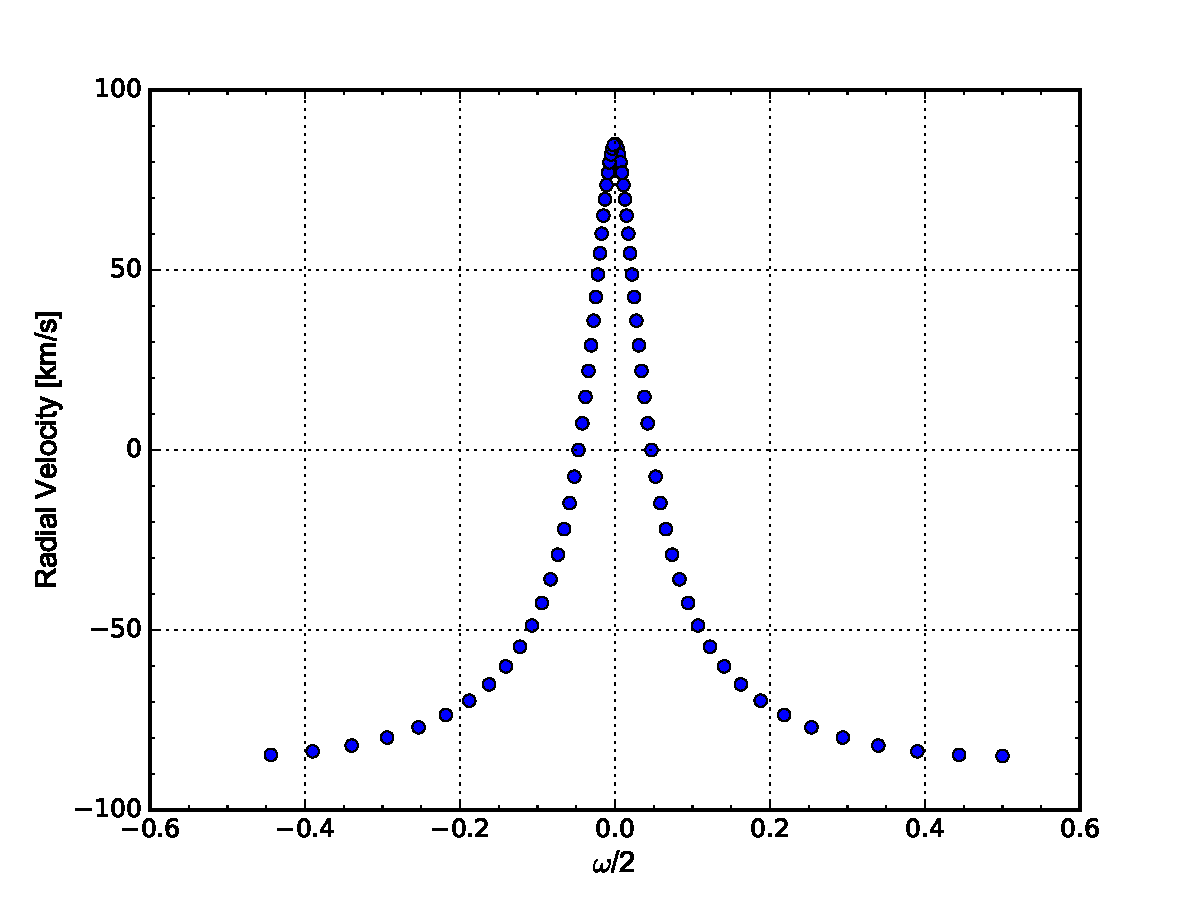
\includegraphics[scale=0.3]{a.pdf}%\quad
  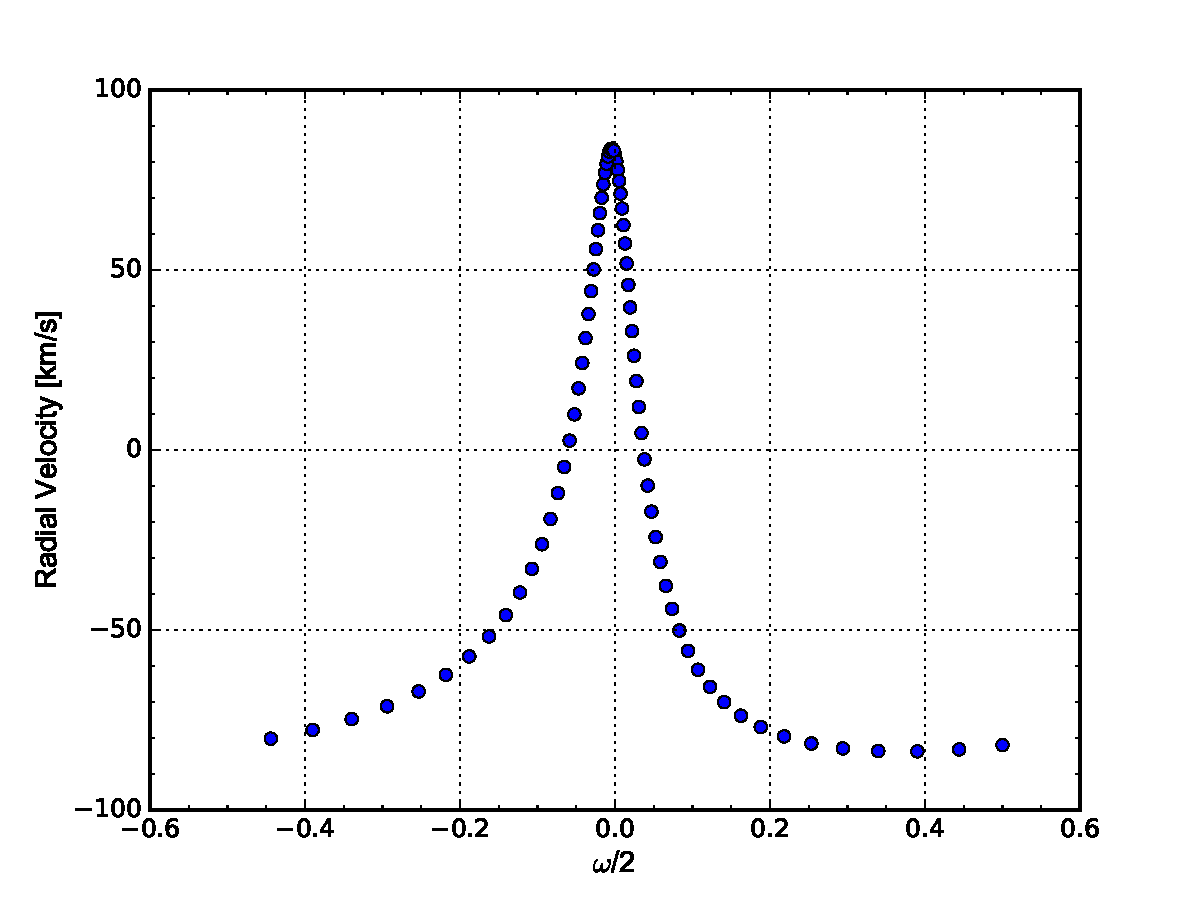
\includegraphics[scale=0.3]{b.pdf}%\quad
  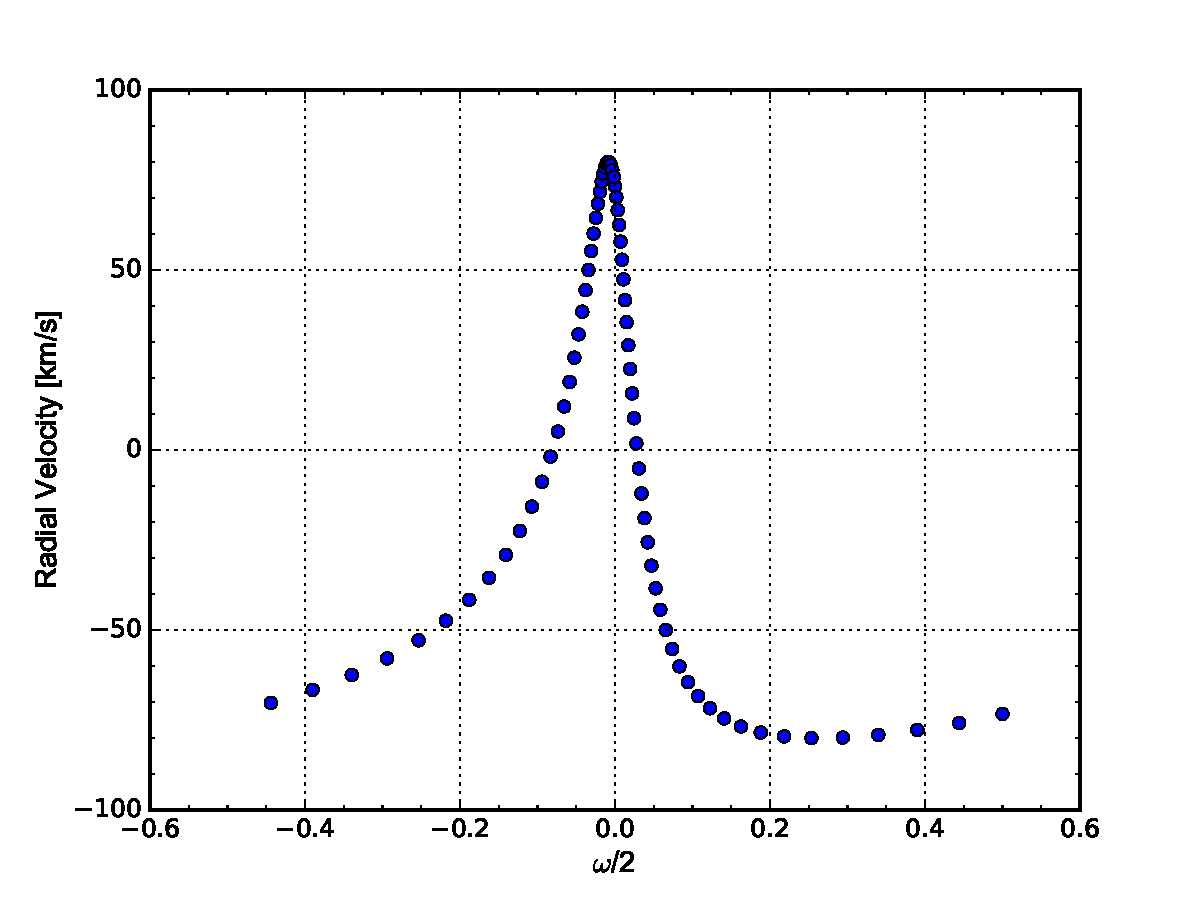
\includegraphics[scale=0.3]{c.pdf} \\%\quad
  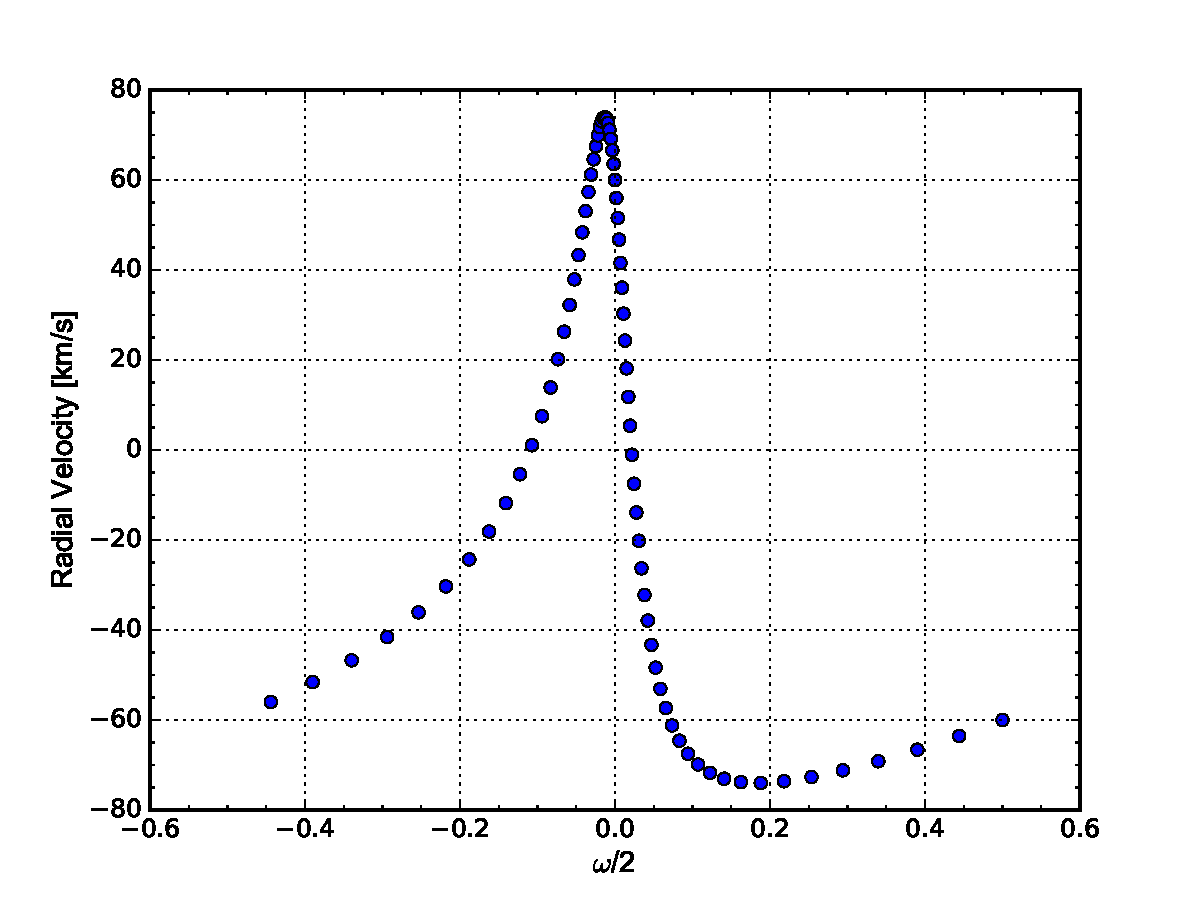
\includegraphics[scale=0.3]{d.pdf}%\quad
  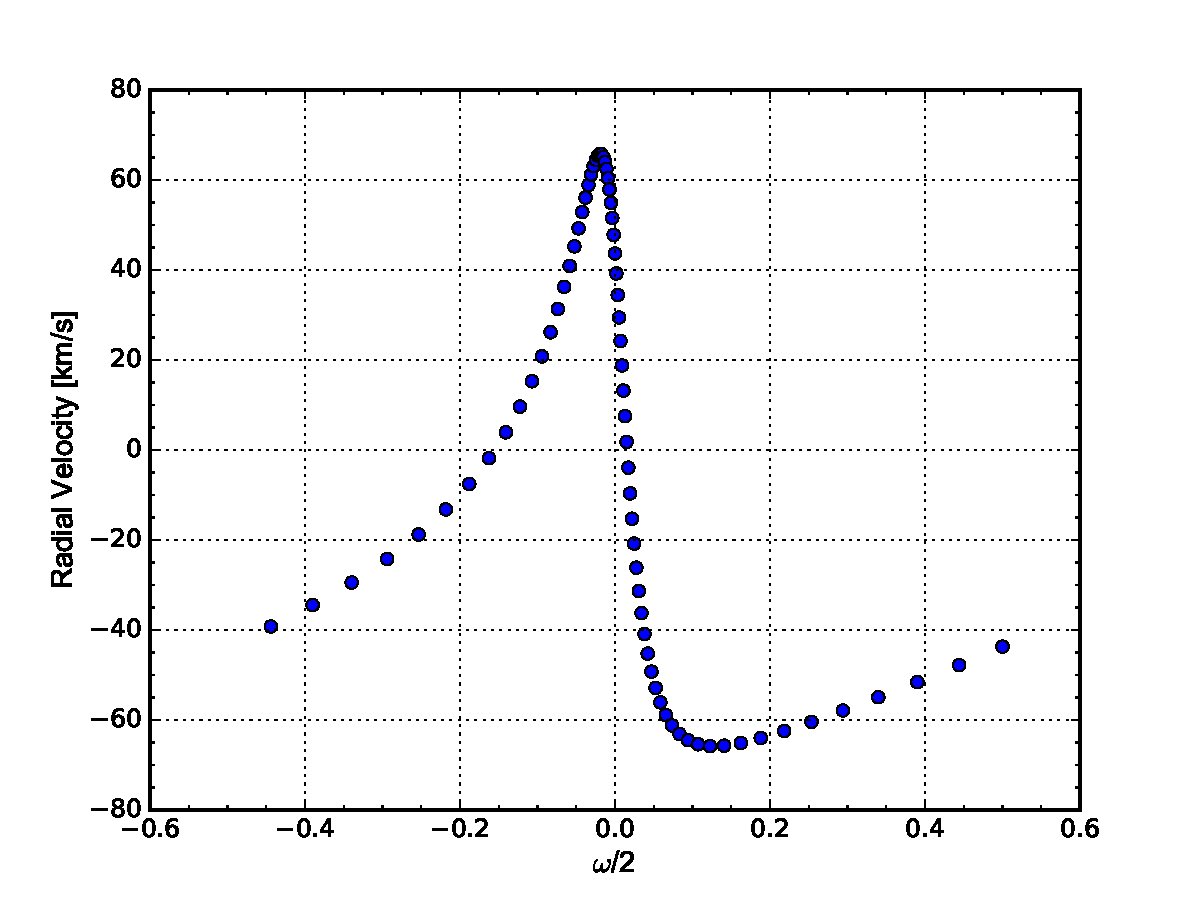
\includegraphics[scale=0.3]{e.pdf}%\quad
  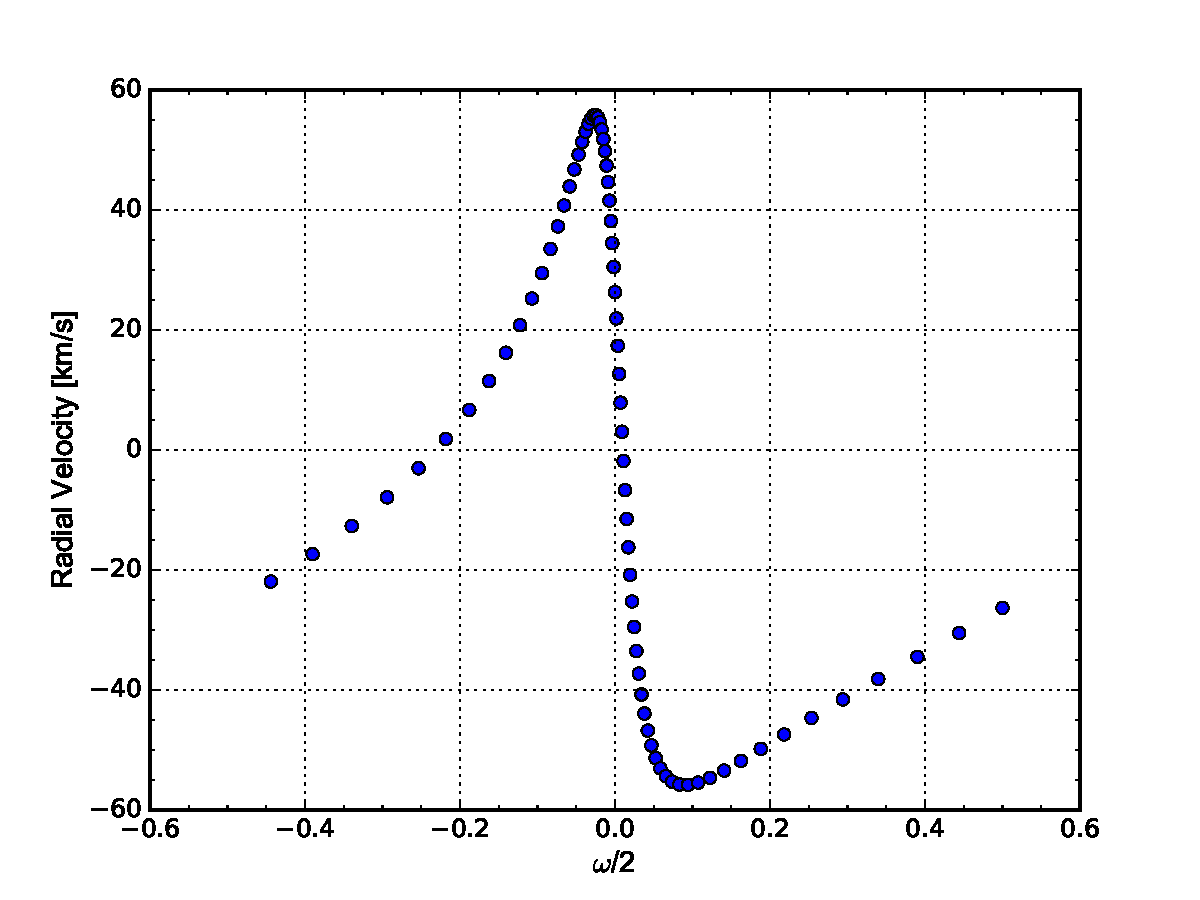
\includegraphics[scale=0.3]{f.pdf} \\%\quad 
  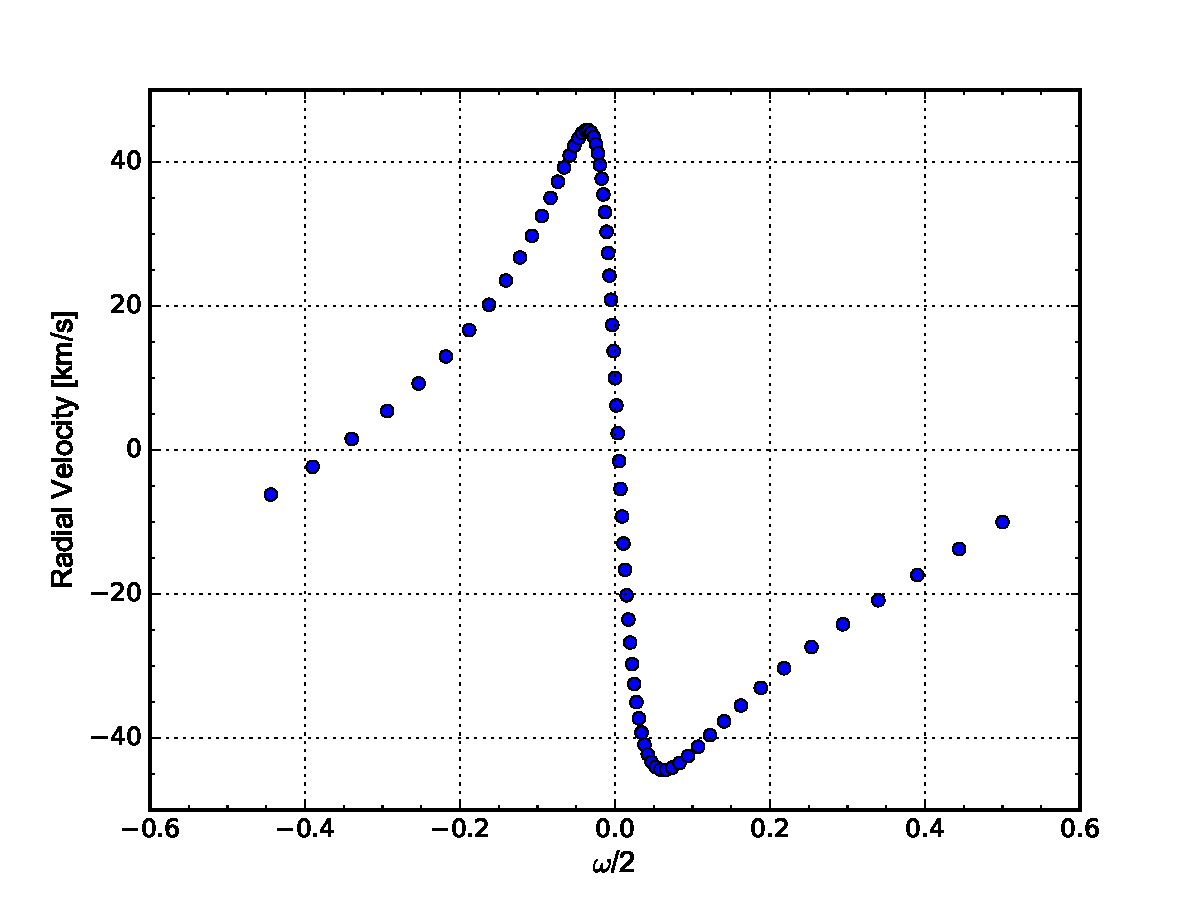
\includegraphics[scale=0.3]{g.pdf}%\quad  
  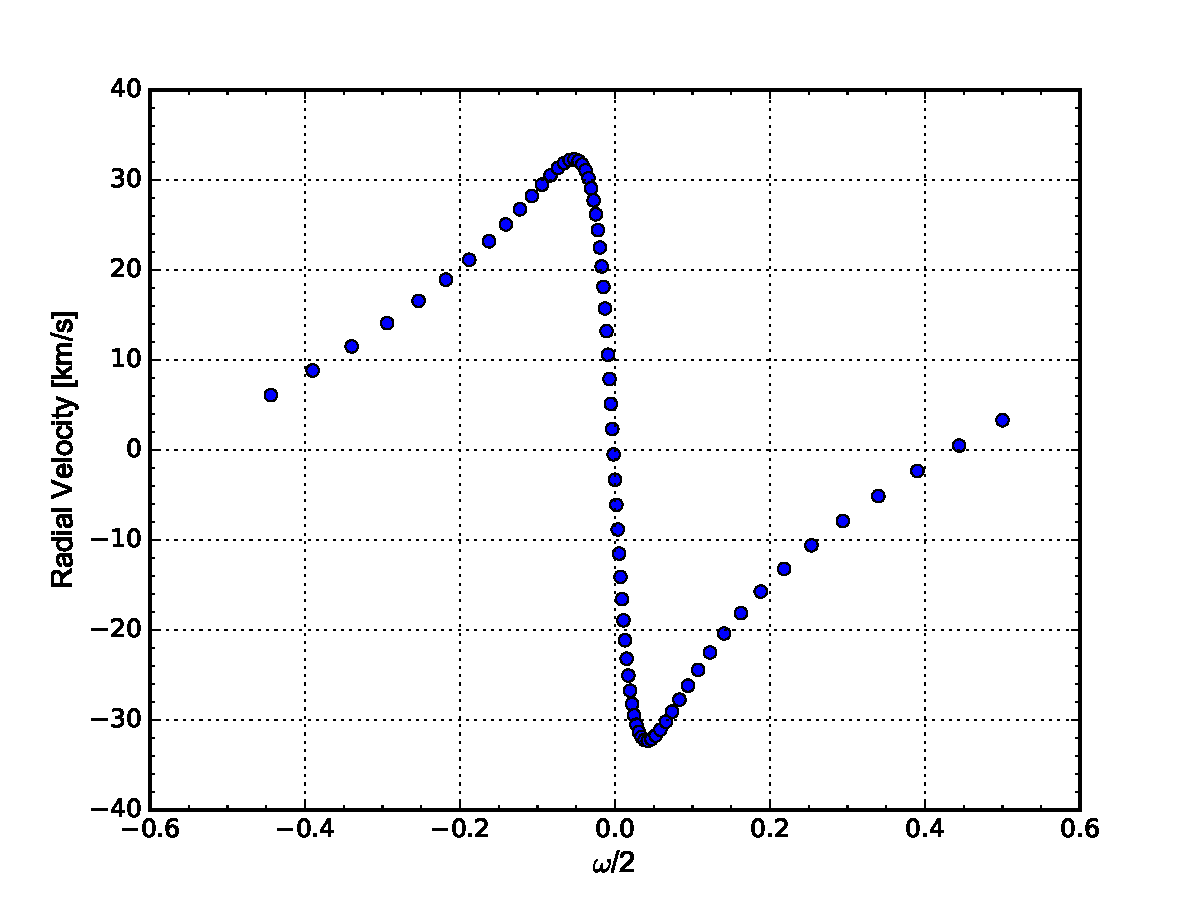
\includegraphics[scale=0.3]{h.pdf}%\quad
  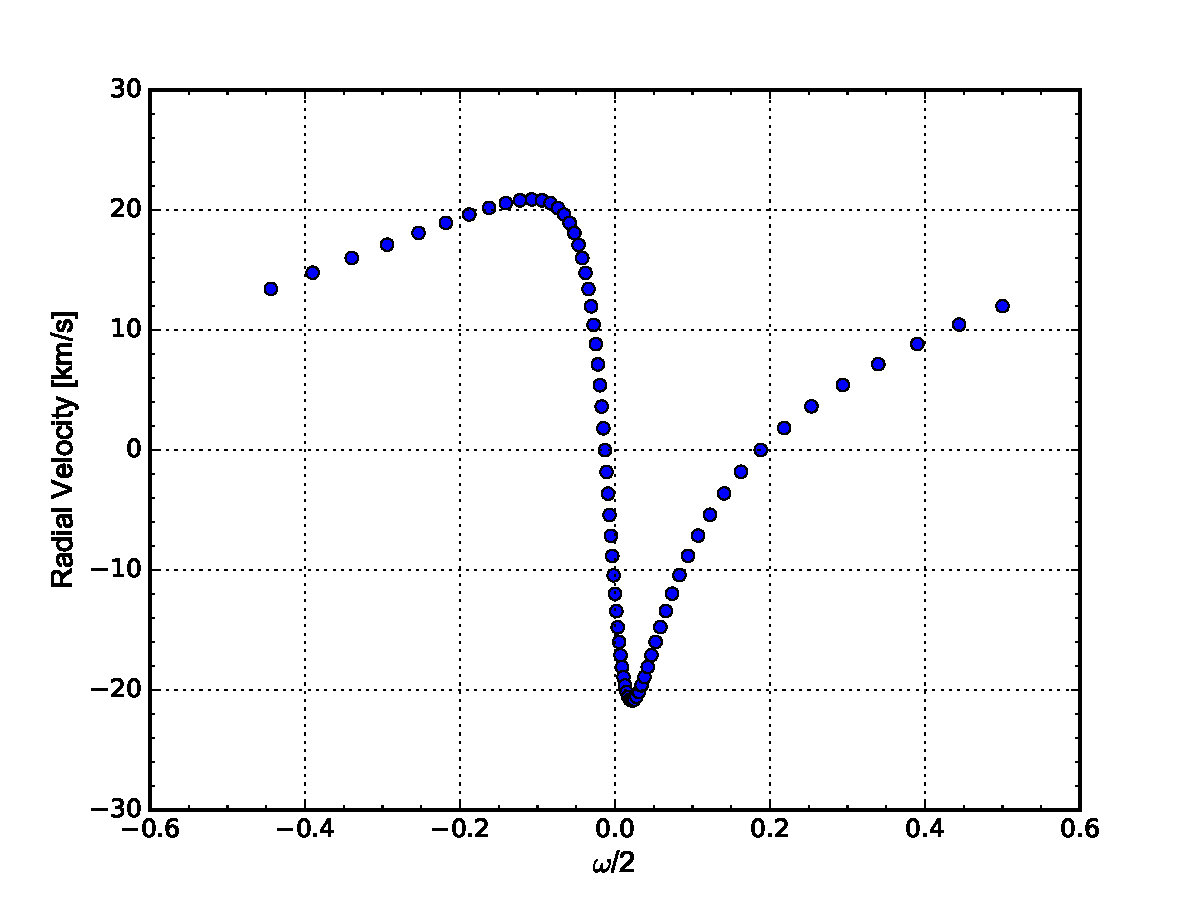
\includegraphics[scale=0.3]{i.pdf}%\quad




  \caption{Elliptical orbits for increasing true anomaly of 5$^\circ$ and periastron of 20$^\circ$ increments.}
  \label{distancevel}
\end{figure*}



\begin{figure*}[ht]
  \centering
  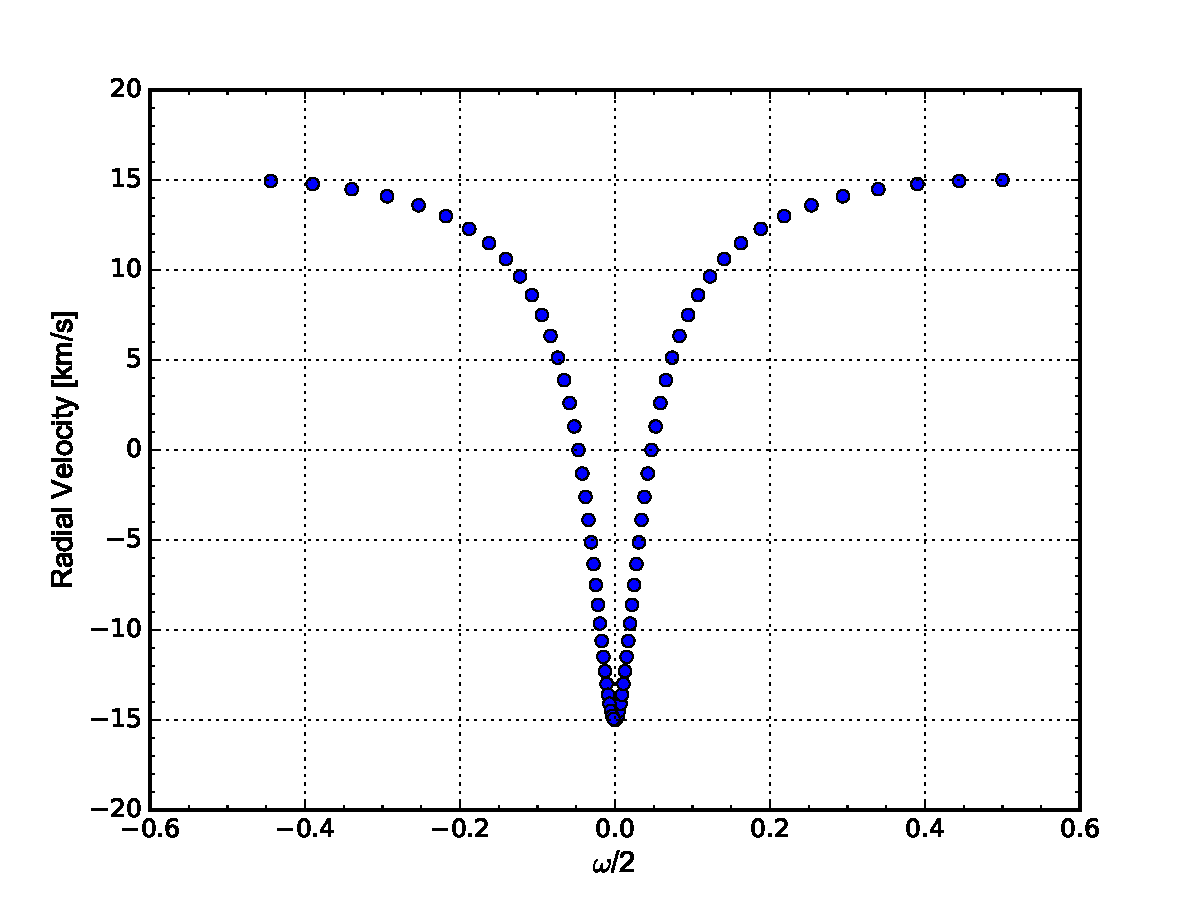
\includegraphics[scale=0.3]{j.pdf}%\quad
  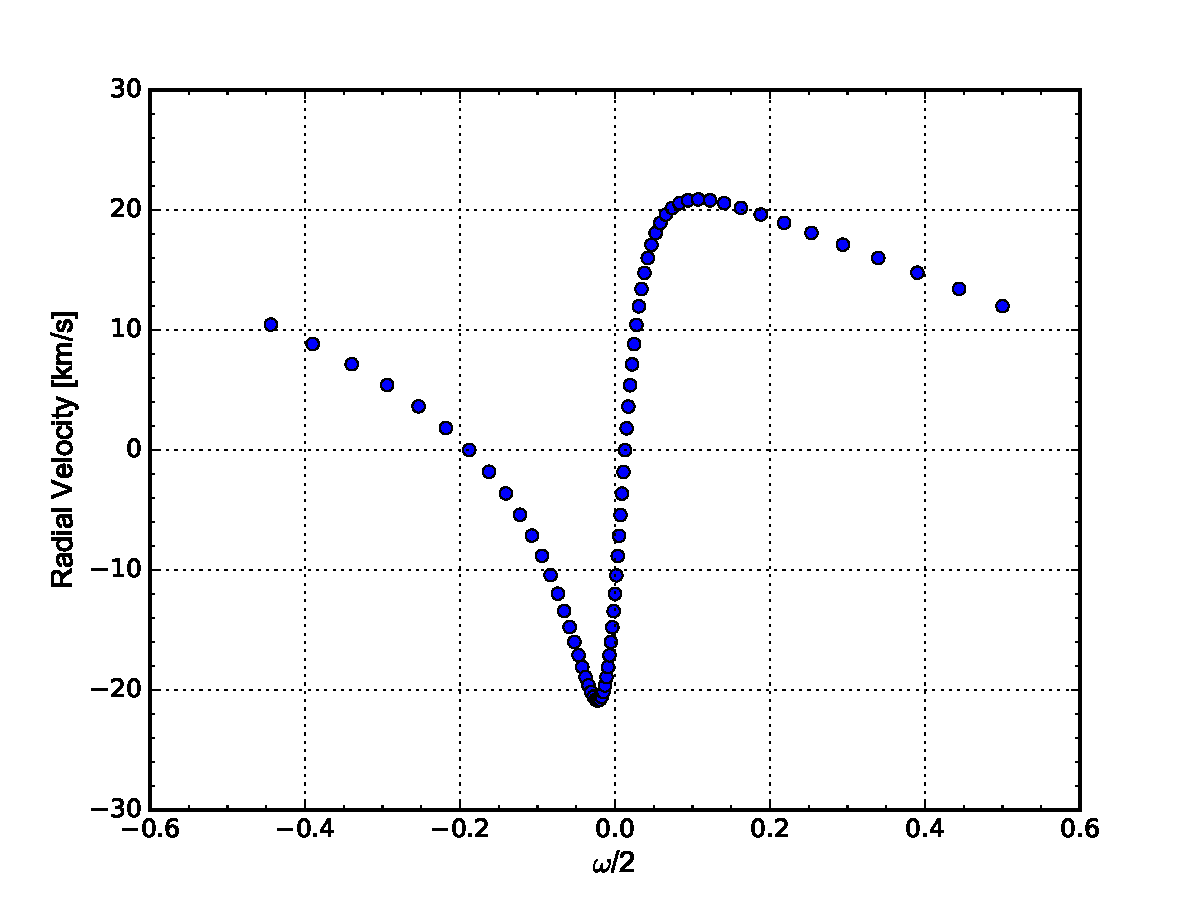
\includegraphics[scale=0.3]{k.pdf}%\quad
  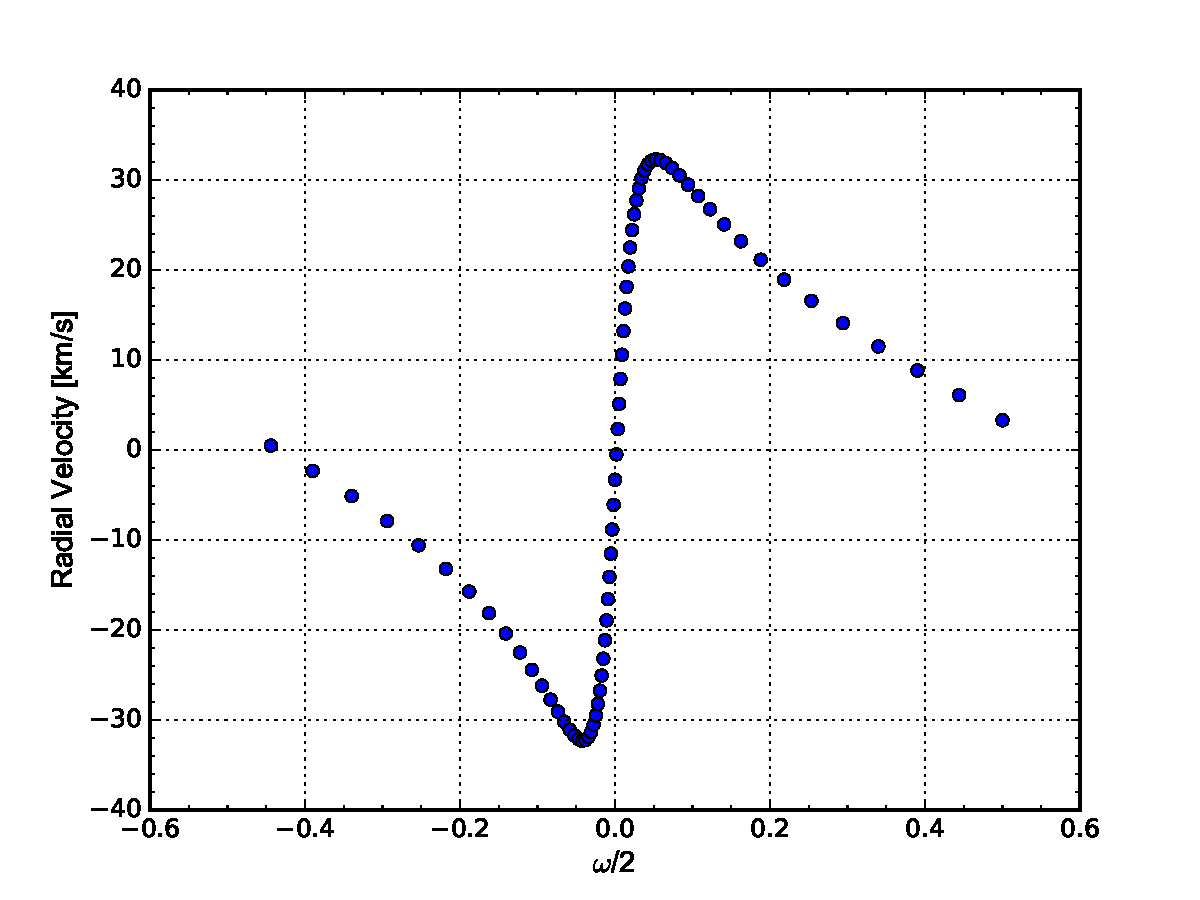
\includegraphics[scale=0.3]{l.pdf} \\%\quad
  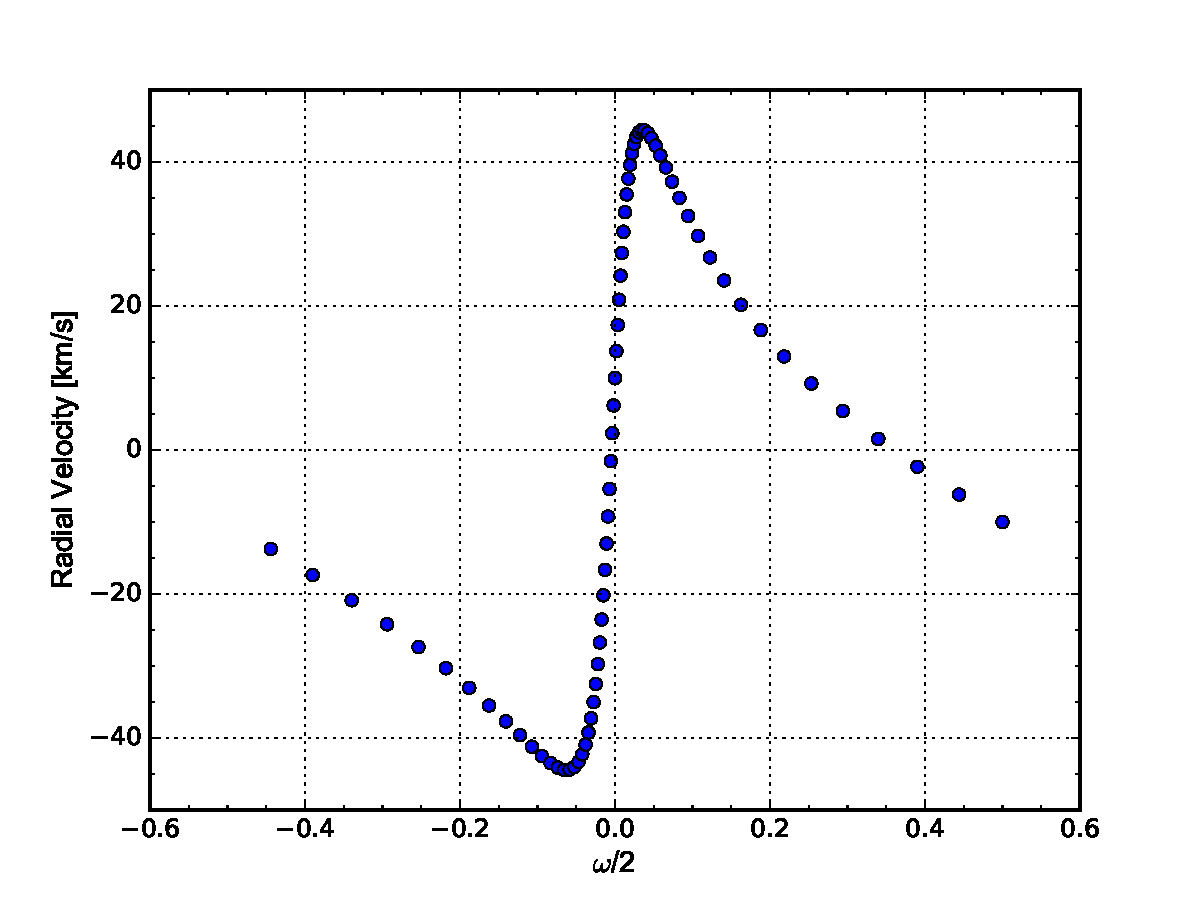
\includegraphics[scale=0.3]{m.pdf}%\quad
  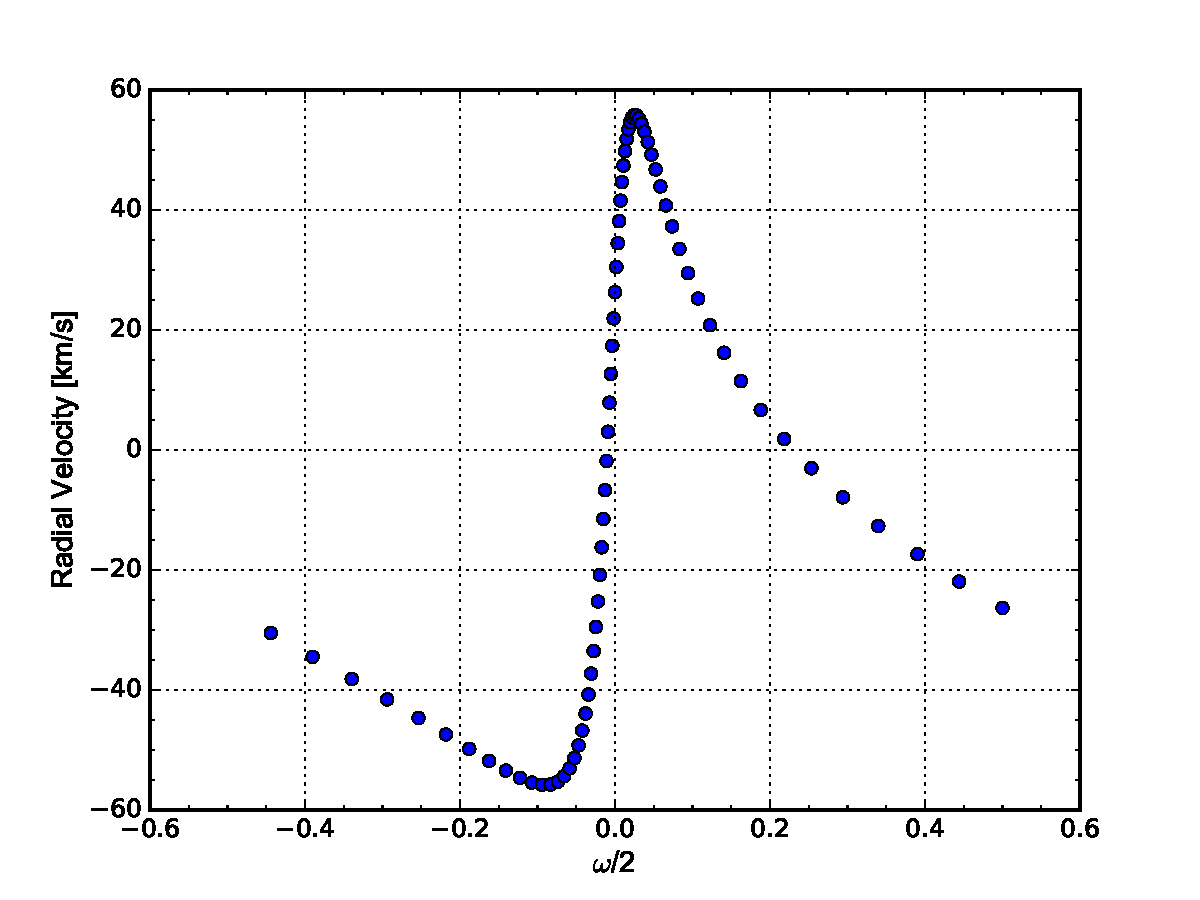
\includegraphics[scale=0.3]{n.pdf}%\quad
  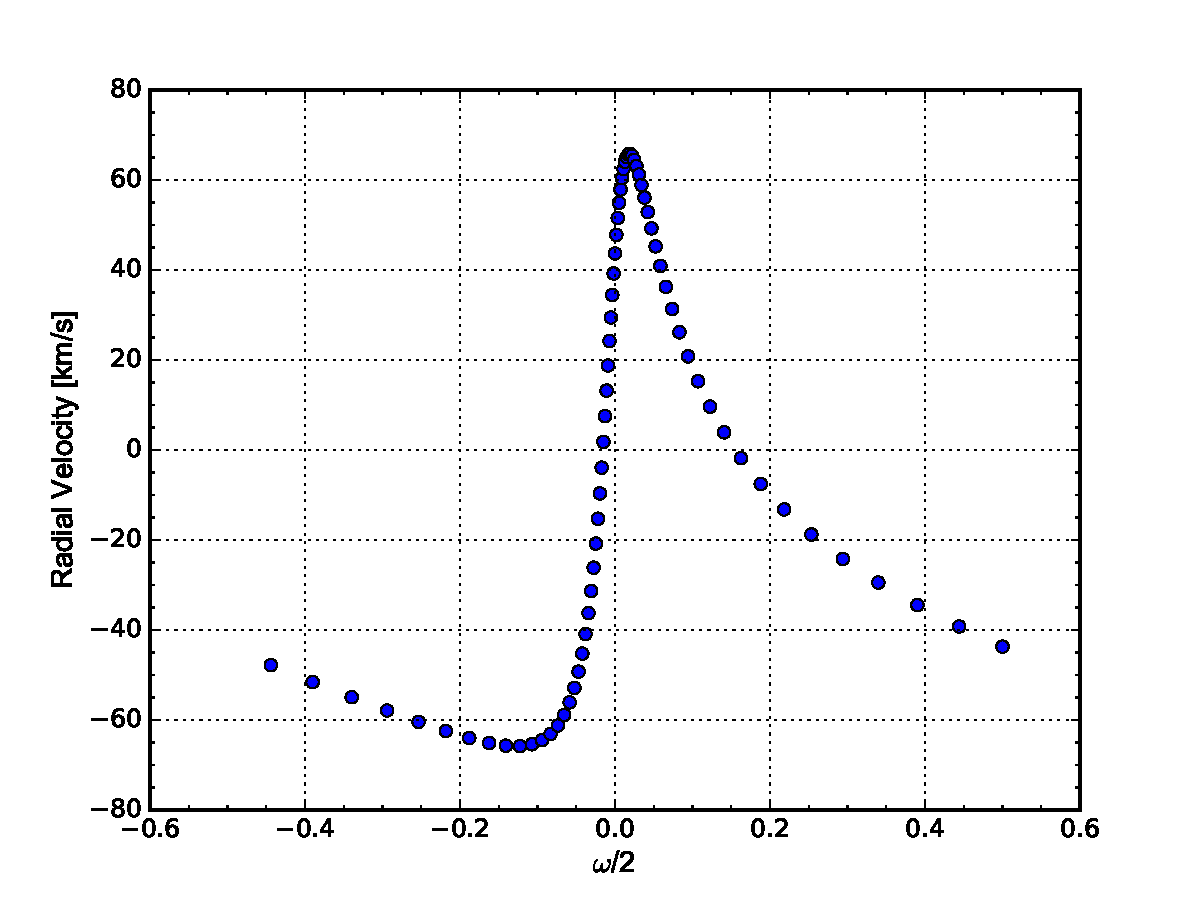
\includegraphics[scale=0.3]{o.pdf} \\%\quad
  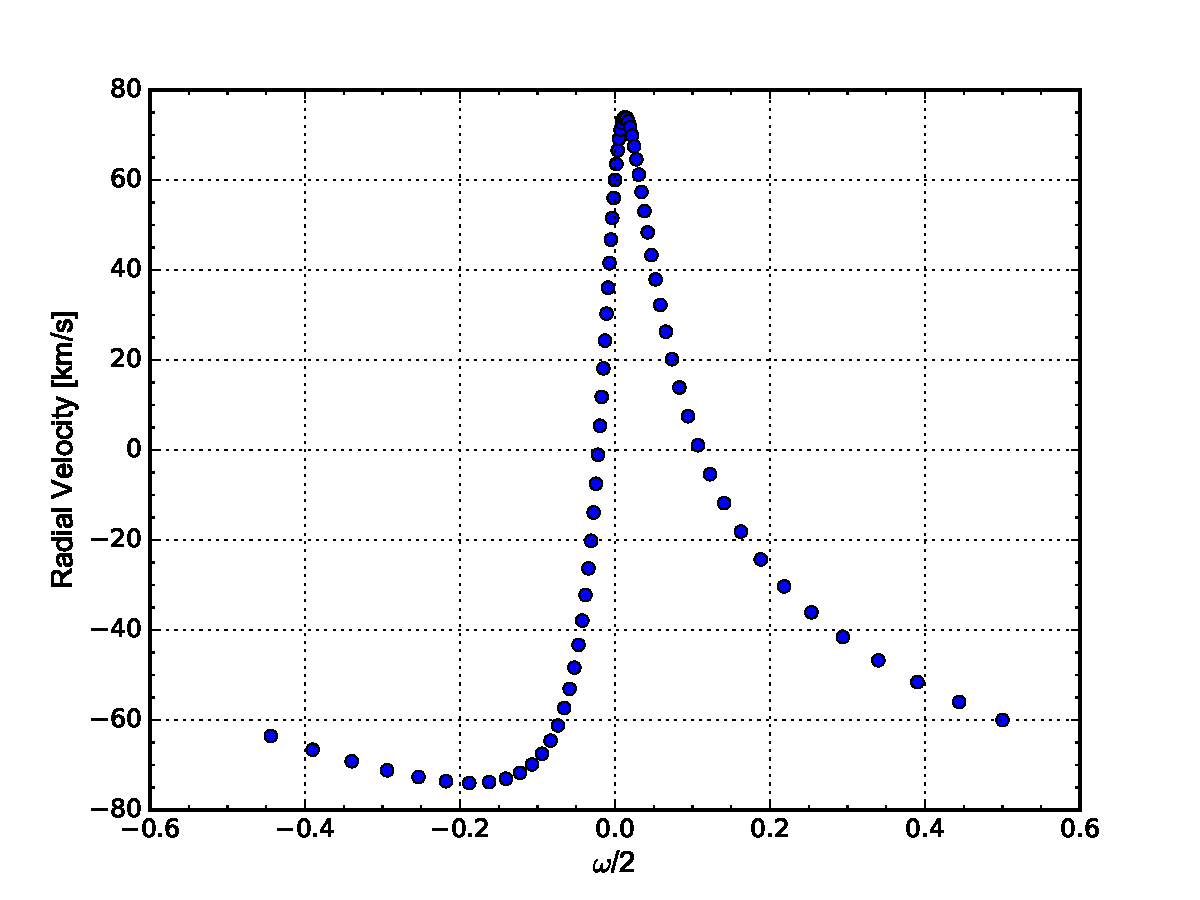
\includegraphics[scale=0.3]{p.pdf}%\quad
  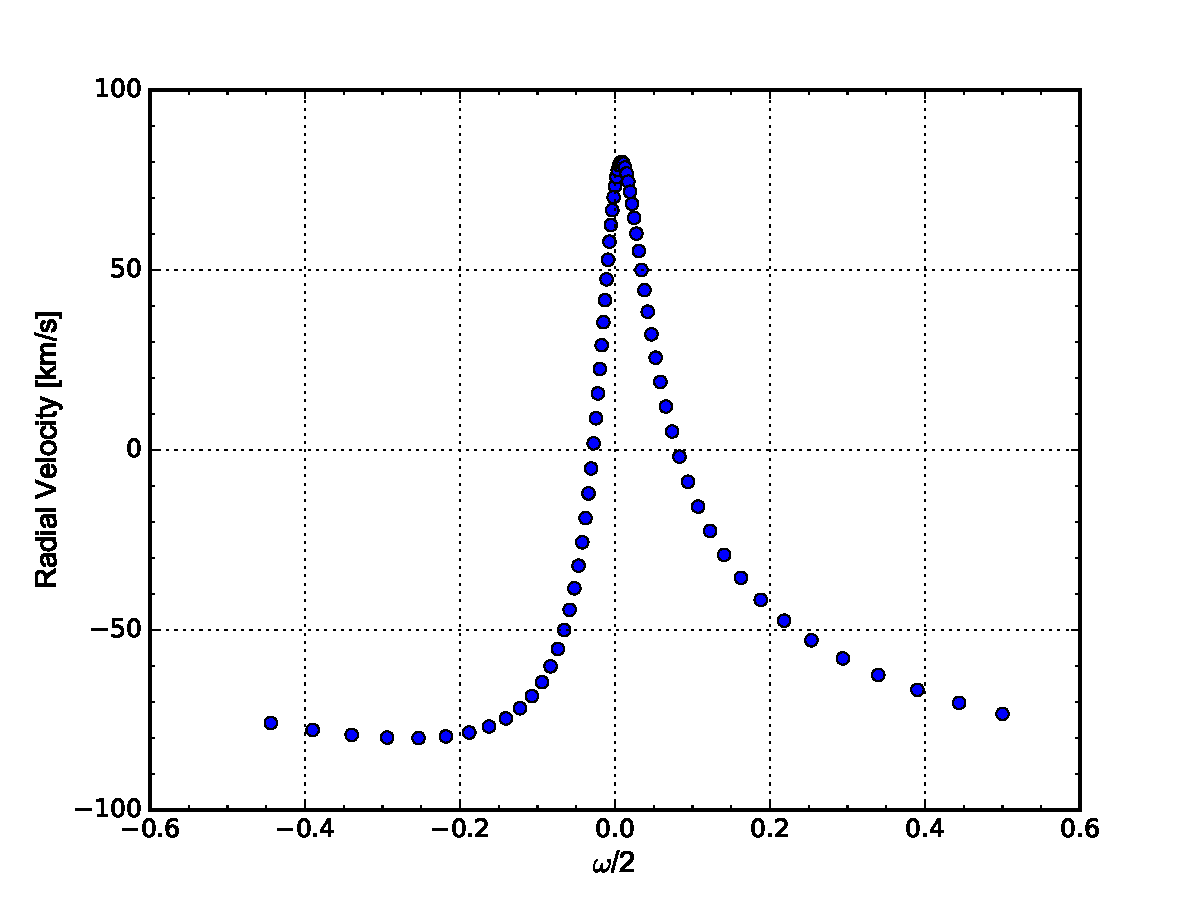
\includegraphics[scale=0.3]{q.pdf}%\quad
  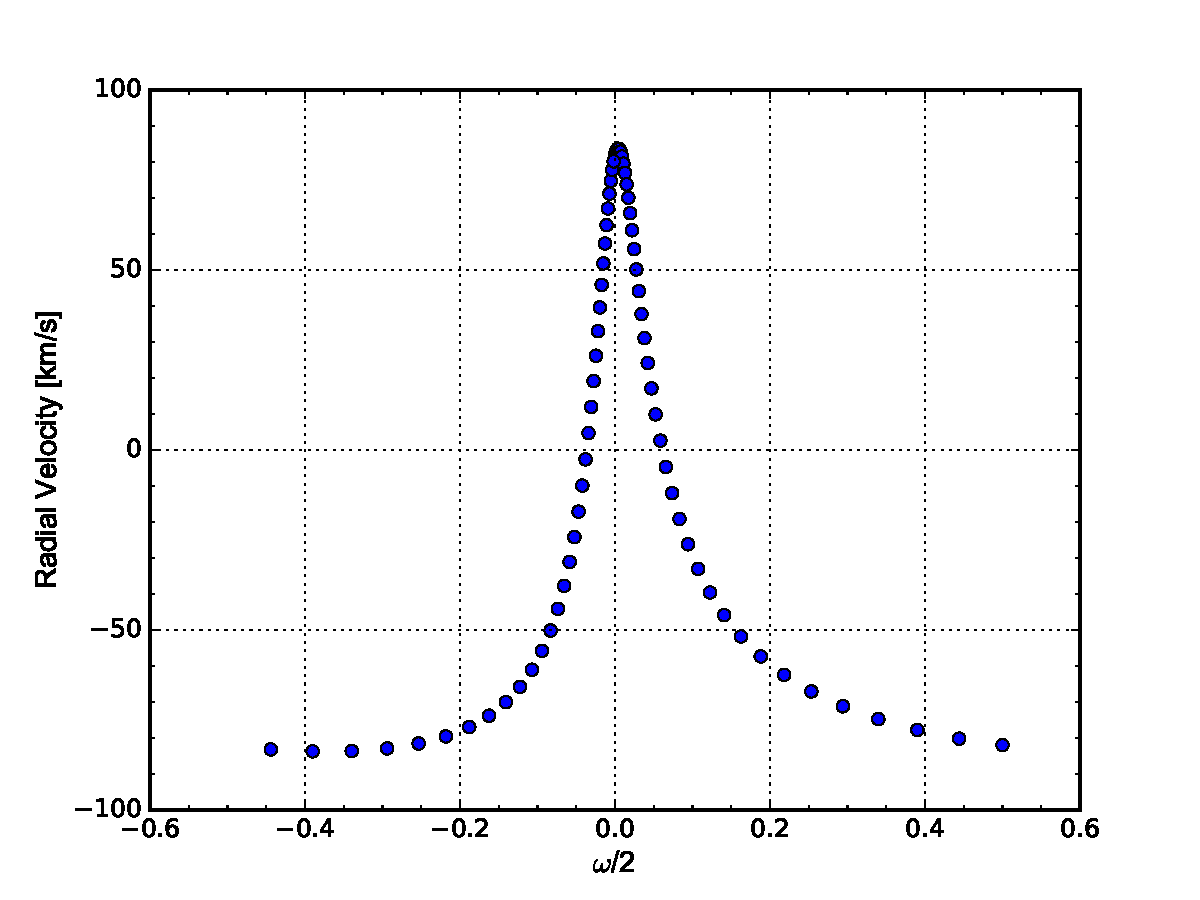
\includegraphics[scale=0.3]{r.pdf}%\quad



  \caption{Elliptical orbits for increasing true anomaly of 5$^\circ$ and periastron of 20$^\circ$ increments.}
  \label{distancevel}
\end{figure*}
%\acknowledgments

\clearpage
\section{3.0 Period Search Using Radial Velocity Data}
The heliocentric radial velocity data is provided in table\,\ref{spectable} in the appendix.
\subsection{Method of Lafler and Kinman}



\begin{figure*}[ht]
  \centering
  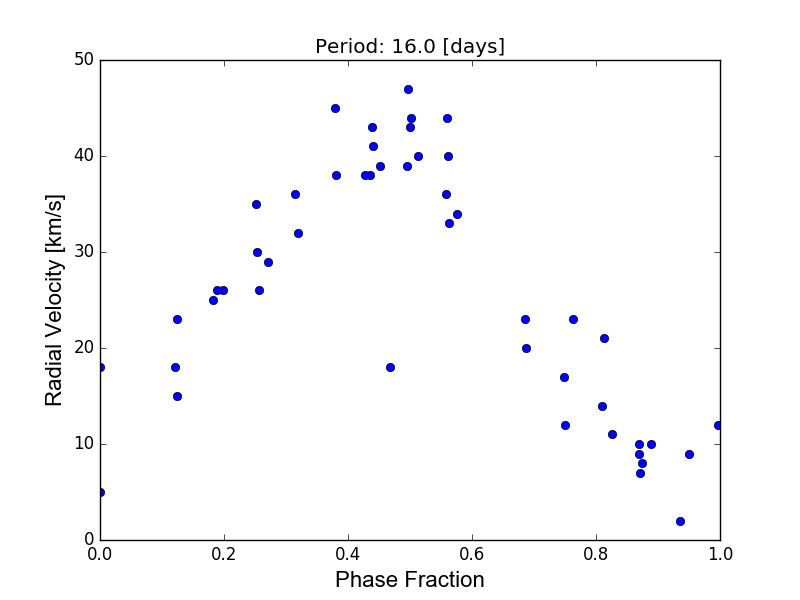
\includegraphics[scale=0.3]{period2.png}%\quad
  \caption{The best period plot using period increments from 3 to 40 days.}
  \label{lafler}
\end{figure*}

\begin{equation}
\Theta = \frac{\sum_i (m_i - m_{i+1})^2}{\sum_i (m_i - \bar{M})^2}
\label{lafeqn}
\end{equation}


Figure\,\ref{lafler} was generated using the Lafler and Kinman method, equation\,\ref{lafeqn}, to find the period. The period that yielded the lowest $\Theta$ value was 16.0\,days. The 16\,day period yields a semi-amplitude radial velocity of 46.6146\,km/s. This is compared to the SIMBAD radial velocity for NGC 2346, which was 47\,km/s. 

\subsection{Lomb-Scargle Method}

The Fast Lomb-Scargle method outlined in \textit{gatspy} yielded a period between 3 and 40 days of 15.9925318331. This result agrees within 0.1 of the Lafler and Kinman method, which produced a period of 16\,days.



\clearpage
\section{Appendix}


\begin{lstlisting}[language=Python, caption=Python example]
import datetime
import numpy as np
import matplotlib.pyplot as plt
from astropy.stats import sigma_clip
from numpy import mean
from astropy.io import fits as fits
from astropy import units as u
from astropy.coordinates import SkyCoord
from matplotlib.patches import Rectangle
from astropy.coordinates import Angle
from scipy import ndimage
from astropy import units as u
import ccdproc
import pyfits
from matplotlib.colors import LogNorm
from astropy.stats import LombScargle
import astropy.units as u
from gatspy import periodic

JD = []
V = []

JD = np.genfromtxt("rv2346.dat", usecols = 0)
V = np.genfromtxt("rv2346.dat", usecols = 1)

#period = np.arange(15, 17, 0.1)
#period = np.arange(16, 17, 0.0000000000001)
'''
for i in period:
  plt.clf()
  phase_frac = (JD - JD[0])\%i/i
  plt.plot(phase_frac, V, "o")
  plt.xlabel('Phase Fraction', fontname="Arial", fontsize = 16)
  plt.ylabel('Radial Velocity [km/s]', fontname="Arial", fontsize = 16)
  plt.title("Period: "+str(i)+" [days]")
  plt.show()
'''
plt.clf()
model = periodic.LombScargleFast(fit_period=True)
model.optimizer.period_range = (3.0, 40.0)
model.fit(JD, V, None)
print(model.best_period)
\end{lstlisting}
\clearpage

\begin{deluxetable}{cc}
\tablecaption{Radial Velocities.}
\tablecolumns{2}
\tablenum{1}
\tablewidth{0pt}
\tablehead{
\colhead{Julian Date}  & \colhead{Radial Velocity}\\
\colhead{} & \colhead{[km/s]} }
\centering
\startdata
43138.66  &  5.0\\
43140.654 & 23.0\\
43141.829 & 26.0\\
43142.775 & 26.0\\
43143.702 & 36.0\\
43144.758 & 38.0\\
43146.664 & 43.0\\
43147.651 & 40.0\\
43200.559 & 10.0\\
43878.7   & 30.0\\
43879.778 & 32.0\\
43880.731 & 45.0\\
43881.689 & 43.0\\
43881.717 & 41.0\\
43882.698 & 44.0\\
43883.673 & 33.0\\
43885.651 & 20.0\\
43886.657 & 12.0\\
43887.661 & 21.0\\
43888.647 &  8.0\\
43890.668 & 18.0\\
43892.643 & 15.0\\
43893.675 & 26.0\\
43894.682 & 35.0\\
43914.591 & 39.0\\
43915.598 & 36.0\\
43920.569 &  9.0\\
44137.879 & 39.0\\
44138.859 & 40.0\\
44139.868 & 34.0\\
44142.869 & 23.0\\
44143.874 & 11.0\\
44144.87  & 10.0\\
44145.861 &  9.0\\
44265.633 & 38.0\\
44266.6   & 47.0\\
44267.625 & 44.0\\
44269.615 & 23.0\\
44270.628 & 17.0\\
44271.608 & 14.0\\
44272.585 &  7.0\\
44273.631 &  2.0\\
44274.603 & 12.0\\
44276.607 & 18.0\\
44277.571 & 25.0\\
44377.486 & 38.0\\
56967.004 & 29.0\\
56970.135 & 18.0
\enddata
%\tablenotetext{a}{At exposure start.}
\tablecomments{Heliocentric radial velocity against Julian Date. Note that the number 2400000 is subtracted from the provided Julian Date.}
\label{spectable}
\end{deluxetable}

\vspace{5mm}





%% Appendix material should be preceded with a single \appendix command.
%% There should be a \section command for each appendix. Mark appendix
%% subsections with the same markup you use in the main body of the paper.

%% Each Appendix (indicated with \section) will be lettered A, B, C, etc.
%% The equation counter will reset when it encounters the \appendix
%% command and will number appendix equations (A1), (A2), etc.


%% The reference list follows the main body and any appendices.
%% Use LaTeX's thebibliography environment to mark up your reference list.
%% Note \begin{thebibliography} is followed by an empty set of
%% curly braces.  If you forget this, LaTeX will generate the error
%% "Perhaps a missing \item?".
%%
%% thebibliography produces citations in the text using \bibitem-\cite
%% cross-referencing. Each reference is preceded by a
%% \bibitem command that defines in curly braces the KEY that corresponds
%% to the KEY in the \cite commands (see the first section above).
%% Make sure that you provide a unique KEY for every \bibitem or else the
%% paper will not LaTeX. The square brackets should contain
%% the citation text that LaTeX will insert in
%% place of the \cite commands.

%% We have used macros to produce journal name abbreviations.
%% \aastex provides a number of these for the more frequently-cited journals.
%% See the Author Guide for a list of them.

%% Note that the style of the \bibitem labels (in []) is slightly
%% different from previous examples.  The natbib system solves a host
%% of citation expression problems, but it is necessary to clearly
%% delimit the year from the author name used in the citation.
%% See the natbib documentation for more details and options.


\end{document}

%% End of file `sample.tex'.
